\documentclass[12pt,a4paper]{article}
\usepackage{ctex}
\usepackage{amsmath,amscd,amsbsy,amssymb,latexsym,url,bm,amsthm}
\usepackage{epsfig,graphicx,subfigure}
\usepackage{enumitem,balance}
\usepackage{wrapfig}
\usepackage{mathrsfs,euscript}
\usepackage[usenames]{xcolor}
\usepackage{hyperref}
\usepackage[vlined,ruled,linesnumbered]{algorithm2e}
\hypersetup{colorlinks=true,linkcolor=black}

\newtheorem{theorem}{Theorem}
\newtheorem{lemma}[theorem]{Lemma}
\newtheorem{proposition}[theorem]{Proposition}
\newtheorem{corollary}[theorem]{Corollary}
\newtheorem{exercise}{Exercise}
\newtheorem*{solution}{Solution}
\newtheorem{definition}{Definition}
\theoremstyle{definition}

\renewcommand{\thefootnote}{\fnsymbol{footnote}}

\newcommand{\postscript}[2]
 {\setlength{\epsfxsize}{#2\hsize}
  \centerline{\epsfbox{#1}}}

\renewcommand{\baselinestretch}{1.0}

\setlength{\oddsidemargin}{-0.365in}
\setlength{\evensidemargin}{-0.365in}
\setlength{\topmargin}{-0.3in}
\setlength{\headheight}{0in}
\setlength{\headsep}{0in}
\setlength{\textheight}{10.1in}
\setlength{\textwidth}{7in}
\makeatletter \renewenvironment{proof}[1][Proof] {\par\pushQED{\qed}\normalfont\topsep6\p@\@plus6\p@\relax\trivlist\item[\hskip\labelsep\bfseries#1\@addpunct{.}]\ignorespaces}{\popQED\endtrivlist\@endpefalse} \makeatother
\makeatletter
\renewenvironment{solution}[1][Solution] {\par\pushQED{\qed}\normalfont\topsep6\p@\@plus6\p@\relax\trivlist\item[\hskip\labelsep\bfseries#1\@addpunct{.}]\ignorespaces}{\popQED\endtrivlist\@endpefalse} \makeatother

\begin{document}
\noindent

%========================================================================
\noindent\framebox[\linewidth]{\shortstack[c]{
\Large{\textbf{Lab07-Network Flow}}\vspace{1mm}\\
CS214-Algorithm and Complexity, Xiaofeng Gao, Spring 2019.}}


\begin{center}
\footnotesize{\color{red}$*$ If there is any problem, please contact TA Mingran Peng.}\par
% Please write down your name, student id and email.
\footnotesize{\color{blue}$*$ Name:\underline{��ѩ��}  \quad Student ID: \underline{515030910347}\quad Email:\underline{13487426939@qq,com} }
\end{center}
\begin{enumerate}

    \item
    \begin{solution}
    The following is the process of solution.\\
    The \textbf{way(1)} to solve this problem: at first, we can find the maximum distance from one vertex s to other vertexes by SPFA. then traversal all the vertexes to find maximum distance in the network.\\
    $\bullet$ Find maximum distance  in all  vertexes.\\
    \begin{algorithm}[H]
    \KwIn{All the vertexes of G(V,E)}
    \KwOut{The maximum distance in the network.}
    \caption{Maximum distance.}
    $maximum \leftarrow 0$;\\
    \For{\textbf{each}  u $\epsilon$ \textbf{V}}{
            $maximum \leftarrow SPFA(u);$\\
    }
    \Return{maximum};
    \end{algorithm}
    $\bullet$ Find the maximum distance from s(start vertex) to other vertex.\\
    \begin{algorithm}[H]
     \KwIn{Computer s(start), and  an undirected Graph $G=(V,E)$ represent the relation of computer(connected(delay i) and unconnected(assume delay 0)). vertex s,t $\epsilon$ \textbf{V}.}
    \KwOut{The maximum time needed to send message other computers by vertex s.}
    \caption{SPFA(s) algorithm(maximum).}
    $max(s) \leftarrow 0;$
    \For{\textbf{each}  u $\epsilon$ \textbf{V}}{
           $DIST(u)\leftarrow  0 ;$\\
           $in\_queue[i]\leftarrow false;$\\
    }
    $Q.PUSH(s);$(Using a queue Q to do SPFA.)\\
    $in\_queue[s]\leftarrow true;$(s in queue)\\
    \While{Q is not empty}{
            $u \leftarrow Q.POP()$;\\
            $in\_queue[u] \leftarrow false$;(u out of Q)\\
            \For{\textbf{each} (u,v) $\epsilon$ \textbf{E}}{
                   \If{$DIST[v] < DIST[u]+t_{i}(u,v)$}{
                             $DIST[v] \leftarrow DIST[u]+t_{i}(u,v);$\\
                             \If{$DIST[v]>max(s)$}{
                                     $max \leftarrow DIST[v];$\\
                             }
                             \If{v is not in queue}{
                                     $Q.PUSH(v)$;\\
                                     $in\_queue[v] \leftarrow true;$(v in queue)\\
                             }
                   }
            }
    }
    \Return{max(s)}
    \end{algorithm}
    \textbf{Time complexity:}\\
    \textbf{Best case:} if all the vertexes are pushed into once by using SPFA,then SFPA time complexity is o(V+E), the time time complexity of finding the maximum distance in network is o(V(V+E)).\\
   \textbf{ Worst case:}  we assume: there are n vertexes${v_{0},v_{1},v_{2},v_{3}\dots v_{n} }$ ,at first we push $v_{0}$ into the queue, when we pop $v_{0}$, in worst case, we should update the $v_{1},v_{2},\dots v_{n}$ ,when we pop $v_{1}$, we should update $v_{2},v_{3}\dots v_{n} $,and so on. in this case,SPFA time complexity
    is becoming o(VE).  So the time time complexity of finding the maximum distance in network is $o(EV^2)$.\\
    \\
    The \textbf{way(2)} to solve this problem: we can use Floyd-Warshall Algorithm.\\
     \begin{algorithm}[H]
       \KwIn{An undirected Graph $G=(V,E)$ represent the relation of computer(connected(delay i) and unconnected(assume delay 0)). vertex s,t $\epsilon$ \textbf{V}}
       \KwOut{The maximum distance in the network.}
       \caption{Floyd-Warshall Algorithm}
       \For{\textbf{each} v $\epsilon$ \textbf{V} }{
                \For{\textbf{each} u $\epsilon$ \textbf{V} }{
                            \If{(v,u) $\epsilon$ E}{
                            $EDGE[v][u] \leftarrow (-ti(v,u))$;(use negative to find minimal number)\\
                            }
                            \Else{
                            $EDGE[v][u] \leftarrow 0$;\\
                            }
                 }
       }
       $min \leftarrow 0 $;\\
       \For{ $k \leftarrow 1$ \textbf{ to} n}{
                \For{$i \leftarrow 1$ \textbf{to} n}{
                        \For{$j \leftarrow 1$ \textbf{to} n}{
                                 \If{$EDGE[i][j]>EDGE[i][k]+EDGE[k][j]$}{
                                              $EDGE[i][j] \leftarrow EDGE[i][k]+EDGE[k][j]$;\\
                                  }
                        }
                 }
       }
       \For{$i \leftarrow 1$ \textbf{to} n}{
                        \For{$j \leftarrow 1$ \textbf{to} n}{
                                 \If{$EDGE[i][j]<min$}{
                                              $min \leftarrow EDGE[i][j]$;\\
                                  }
                      }
        }
        $maximum \leftarrow (-min)$;\\
        \Return{maximum};
     \end{algorithm}
     \textbf{Time complexity:} Obviously,  Floyd-Warshall Algorithm time complexity is $o(n^3).$\\
    \end{solution}

\vspace{9cm}
\item
   \begin{solution}
     The following is the process of solution.\\
     \textbf{ab.} In this case,because there exist the cost which is negative, i will use SPFA to solve this problem. and in this problem,we also should know whether there exist a negative circle. So i use an array to count the times of all vertexes are  pushed into queue.If there exist a vertex which is pushed into queue more than n times, there must exist a circle in G(V,E).\\
     \\
    \begin{algorithm}[H]
     \KwIn{Computer s(start) and e(end), and  a directed Graph $G=(V,E)$  represent the cost $w_{i}(u,v)$ from one vertex to another vertex. vertex s,e $\epsilon$ \textbf{V}.}
    \KwOut{The minimum cost from s to e.}
    \caption{SPFA(s) algorithm.}
    \For{\textbf{each}  u $\epsilon$ \textbf{V}}{
           $DIST(u)\leftarrow  \infty;$\\
           $in\_queue[u]\leftarrow false;$\\
           $COUNT[u]=0$;(count the times of vertex is pushed into the queue)\\
    }
    $Q.PUSH(s);$(Using a queue Q to do SPFA.)\\
    $COUNT[s] \leftarrow COUNT[s]+1$;\\
    $in\_queue[s]\leftarrow true;$(s in queue)\\
    \While{Q is not empty}{
            $u \leftarrow Q.POP()$;\\
            $in\_queue[u] \leftarrow false$;(u out of Q)\\
            \For{\textbf{each} (u,v) $\epsilon$ \textbf{E}}{
                   \If{$DIST[v] > DIST[u]+t_{i}(u,v)$}{
                             $DIST[v] \leftarrow DIST[u]+t_{i}(u,v);$\\
                             \If{v is not in queue}{
                                     $Q.PUSH(v)$;\\
                                     $in\_queue[v] \leftarrow true;$(v in queue)\\
                                     $COUNT[s] \leftarrow COUNT[s]+1$;\\
                                     \If{$COUNT[s] \geq n$}{
                                             \Return{There exist a negative circle.}\\
                                     }
                             }
                   }
            }
    }
    \Return{$DIST[e]$};\\
    \end{algorithm}
    \textbf{Time complexity:}\\
    \textbf{Best case:} if all the vertexes are pushed into once by using SPFA,time complexity is o(V+E).\\
   \textbf{ Worst case:}  we assume: there are n vertexes ${v_{0},v_{1},v_{2},v_{3}\dots v_{n} }$ ,at first we push $v_{0}$ into the queue, when we pop $v_{0}$, in worst case, we should update the $v_{1},v_{2},\dots v_{n}$ ,when we pop $v_{1}$, we should update $v_{2},v_{3}\dots v_{n} $,and so on. in this case, SPFA time complexity is becoming o(VE).\\
   \\

   \indent \qquad We also can solve this problem by using Bellman-Ford Algorithm.The input and output are same as SPFA.\\
   \begin{algorithm}[H]
     \caption{Bellman-Ford Algorithm.}
     \For {\textbf{each} v $\epsilon$ V}{
             $DIST[v] \leftarrow + \infty$\\;
     }
     $DIST[s] \leftarrow 0$\\
     \For{ $i \leftarrow 1$ to n}{
               \For {\textbf{each} e(u,v) $\epsilon$ E}{
                        \If{ $DIST[v]> DIST[u]+t_{i}(u,v)$}{
                               $DIST[v]=DIST[u]+t_{i}(u,v)$;\\
                        }
               }
     }
     \For {\textbf{each} v $\epsilon$ V}{
             \If{ $DIST[v]> DIST[u]+t_{i}(u,v)$}{
                       \Return{False};\\
              }
     }
     \Return {$DIST[e]$}
   \end{algorithm}
   \indent \qquad \textbf{Time complexity} of Bellman-Ford is $o(VE)$.\\
   \end{solution}
\item

\color{red}(Bonus)\color{black}\\
\indent \qquad In this problem, we can treat slots,lessons,and professors as nodes, construct edges  according to professors' preference, then the question is obvious becoming a maximum problem, so,we can use the Max-Flow to solve this problem.\\
\indent \qquad So, we use blue, red, green nodes to represent slots, professors, lessons, and the flow of two nodes is 1; then we can use Max-Flow strategy to solve this problem.\\
\indent \qquad Then we can use Fort-Fulkerson Algorithm. If there exists augmenting path in the residual graph $G_f$, then we update residual graph $G_f$, repeat until there have no augmenting path.\\
\indent \qquad To update the residual graph, we can use DFS to find a path from s to t, meanwhile we can remember this path so that we can update $G_f$.\\
\indent \qquad The following graph(example) is to show the relation of professors ,slots and lessons.\\
\begin{figure}[htbp]
\begin{minipage}[h]{0.8\textwidth}
\centering
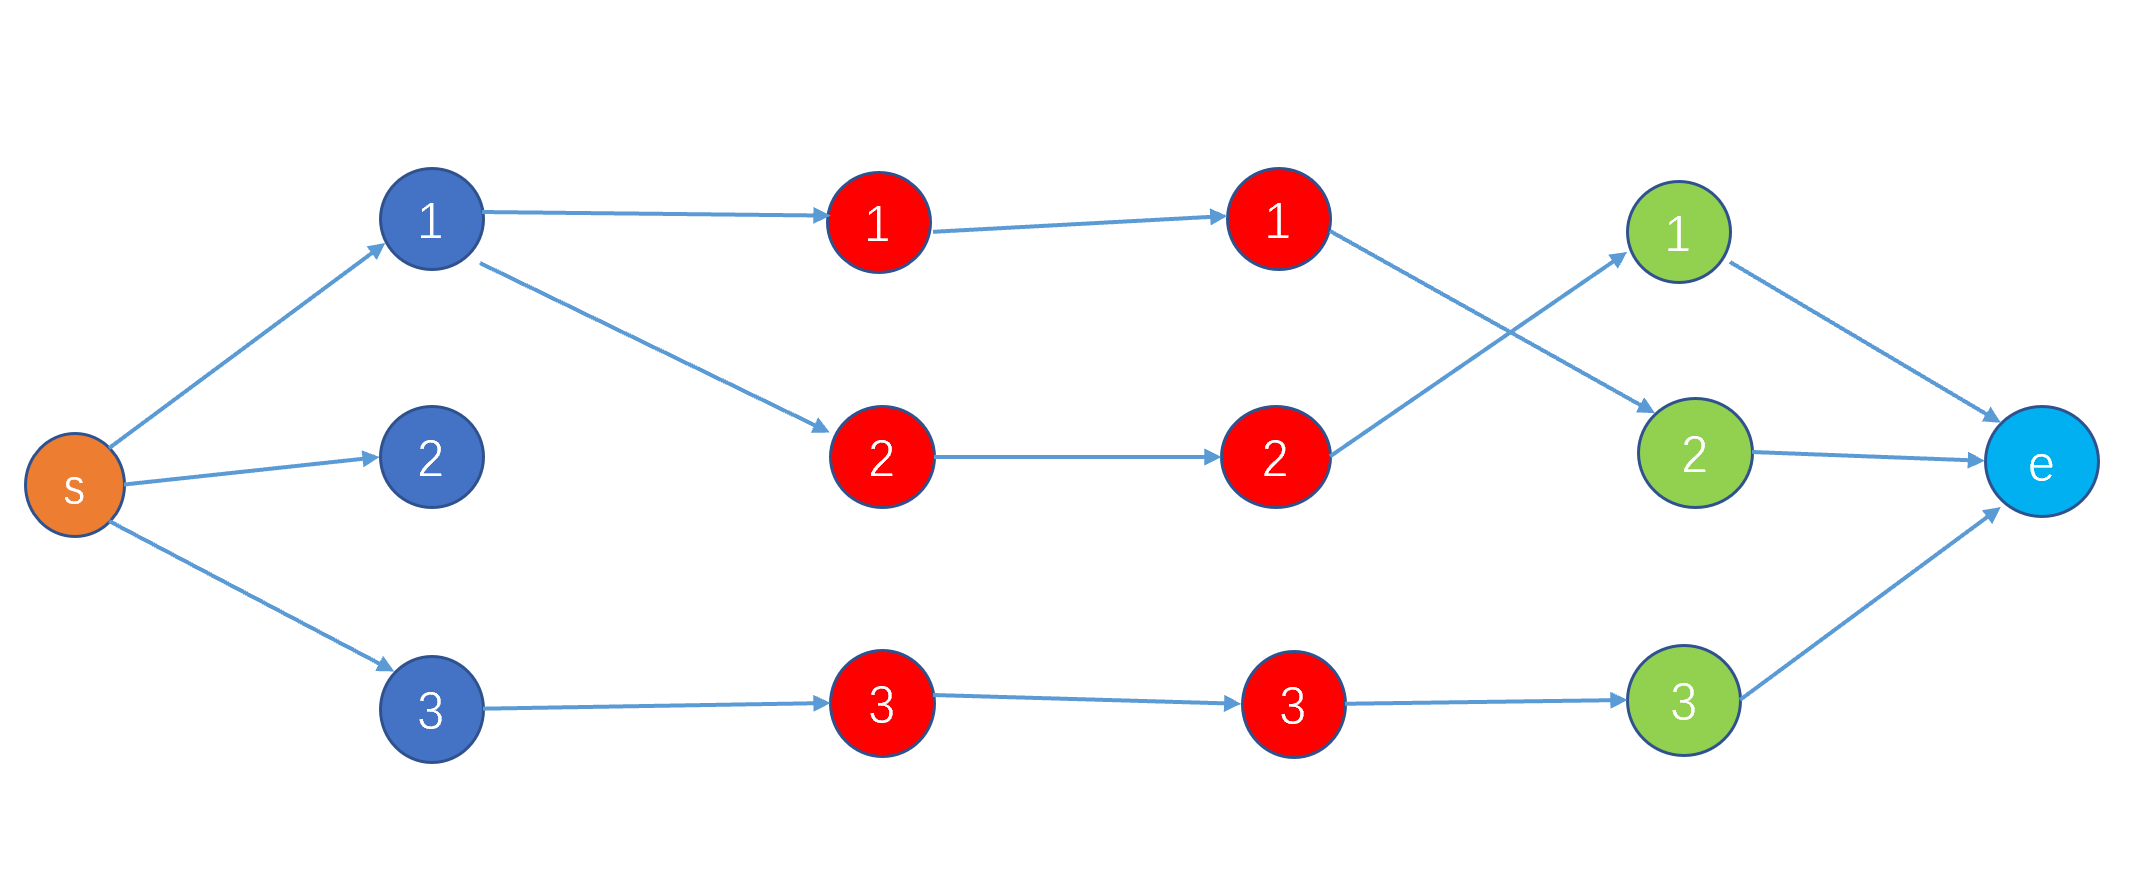
\includegraphics[width=0.9\textwidth]{flow.png}
\caption{The flow of two nodes is 1}
\end{minipage}
\end{figure}

\end{enumerate}

\vspace{20pt}

\textbf{Remark:} You need to include your .pdf and .tex files in your uploaded .rar or .zip file.

%========================================================================
\end{document}
